% ============================================================
%  SmartRide : Project Presentation (Beamer skeleton)
%  B.Tech CSE, TKM Institute of Technology -- Group 14
% ============================================================
\documentclass[aspectratio=169,11pt]{beamer}

\usetheme{Madrid}
\usecolortheme{default}
\setbeamertemplate{navigation symbols}{}

\usepackage[T1]{fontenc}
\usepackage[utf8]{inputenc}
\usepackage{graphicx}
\usepackage{booktabs}
\usepackage{array}
\usepackage{ragged2e}
\usepackage{tikz}
\usetikzlibrary{shapes.geometric,arrows.meta,positioning}

% ---------- Placeholder helper ----------
\newcommand{\placeholder}[1]{\textcolor{gray}{\textit{[#1]}}}

% ---------- Title page info ----------
\title[SmartRide]{SmartRide: Bluetooth-Based Two-Wheeler Ride Logger\\
and Crash Detection System Using ESP32-S3}
\subtitle{Project Phase 1 -- Group 14}
\author[Group 14]{Adarsh Raj \and Muhammed Afsal \and Irfan V \and Rojith Ram}
\institute[TKMIT]{Department of Computer Science and Engineering\\
TKM Institute of Technology, Kollam}
\date{\today}

\begin{document}

% ============================================================
%  1. TITLE & TEAM DETAILS
% ============================================================
\begin{frame}[plain]
  \titlepage
\end{frame}

\begin{frame}{Project Title \& Team Details}
  \textbf{Project Title:} SmartRide: Bluetooth-Based Two-Wheeler Ride Logger
  and Crash Detection System Using ESP32-S3

  \vspace{1em}
  \begin{columns}[T]
    \column{0.55\textwidth}
      \textbf{Team Members}\\[0.4em]
      \begin{tabular}{@{}ll@{}}
        Adarsh Raj      & TKI23CS005 \\
        Muhammed Afsal  & TKI23CS074 \\
        Irfan V         & TKI23CS050 \\
        Rojith Ram      & TKI23CS097 \\
      \end{tabular}
    \column{0.40\textwidth}
      \textbf{Project Guide}\\[0.4em]
      Mrs. Neetha Alex\\[1em]
      \textbf{Project Coordinator}\\[0.4em]
      Dr. Reji R
  \end{columns}
\end{frame}

% ============================================================
%  2. ABSTRACT
% ============================================================
\begin{frame}{Abstract}
  \small\justifying
  SmartRide is a compact, battery-powered on-board unit that turns an ordinary
  two-wheeler or four-wheeler into a connected vehicle by logging every trip and
  detecting crashes in real time. Built around an ESP32-S3 microcontroller, it reads position, speed
  and heading from an ATGM336H-5N multi-constellation GNSS receiver and motion data
  from an MPU6500 six-axis IMU, with an optional ADXL345 accelerometer serving as an
  independent impact channel. A lithium-ion cell protected by a dedicated BMS keeps
  the unit running through the supply interruption of a crash. A selectable vehicle
  mode adapts crash detection to the vehicle type, combining impact magnitude with
  sustained tilt for two-wheelers and with sudden deceleration or rollover for
  four-wheelers, plus post-impact stillness to reject potholes and speed breakers.
  Trip data and
  alerts are streamed over Bluetooth Low Energy to a smartphone app that shows a
  live dashboard, plots routes, stores ride history and issues maintenance
  reminders, with no dependence on a SIM card or cloud services.
\end{frame}

% ============================================================
%  3. PROBLEM STATEMENT
% ============================================================
\begin{frame}{Problem Statement}
  \small
  \begin{block}{Core Problem: Cost and Access}
    Automatic crash detection and trip telematics are available today only in
    premium vehicles or as aftermarket devices that are expensive to buy. Owners
    of the large base of older and budget two- and four-wheelers have no
    affordable option they can retrofit to their existing vehicle.
  \end{block}

  \vspace{0.3em}
  \textbf{Contributing Problems}
  \begin{itemize}
    \item \textbf{Recurring costs:} existing devices need a SIM card, a monthly
      data plan or a paid subscription just to keep working.
    \item \textbf{Closed, proprietary systems:} firmware and apps are locked, so
      users cannot inspect, customise, repair or extend them, and the device
      becomes useless if the vendor drops support.
    \item \textbf{Delayed emergency response:} crash victims, especially lone
      riders and drivers, often get help late because no one is alerted.
    \item \textbf{False alarms:} simple single-threshold detectors trigger on
      potholes and speed breakers, and one fixed rule cannot suit both
      two- and four-wheelers.
    \item \textbf{No trip record:} owners have no data on routes, driving
      behaviour or maintenance due.
    \item \textbf{Privacy and connectivity:} location data is uploaded to
      third-party clouds, and devices fail where mobile coverage is poor.
  \end{itemize}
\end{frame}

% ============================================================
%  4. OBJECTIVES & SCOPE
% ============================================================
\begin{frame}{Objectives \& Scope}
  \begin{columns}[T]
    \column{0.48\textwidth}
      \textbf{Objectives}
      \begin{itemize}
        \item \placeholder{Objective 1}
        \item \placeholder{Objective 2}
        \item \placeholder{Objective 3}
      \end{itemize}
    \column{0.48\textwidth}
      \textbf{Scope}
      \begin{itemize}
        \item \placeholder{Scope item 1}
        \item \placeholder{Scope item 2}
        \item \placeholder{Scope item 3}
      \end{itemize}
  \end{columns}
\end{frame}

% ============================================================
%  5. PROPOSED SOLUTION / METHODOLOGY (max 2 slides)
% ============================================================
\begin{frame}{Proposed Solution / Methodology (1/2)}
  \begin{itemize}
    \item \placeholder{Approach overview}
    \item \placeholder{Key components}
  \end{itemize}
\end{frame}

\begin{frame}{Proposed Solution / Methodology (2/2)}
  \begin{center}
    \placeholder{Insert methodology / block diagram here}
    % \includegraphics[width=0.8\textwidth]{methodology.png}
  \end{center}
\end{frame}

% ============================================================
%  6. PRELIMINARY LITERATURE SURVEY (max 2 slides)
% ============================================================
\begin{frame}{Preliminary Literature Survey (1/2)}
  \small
  \begin{tabular}{@{}p{0.28\textwidth}p{0.32\textwidth}p{0.32\textwidth}@{}}
    \toprule
    \textbf{Paper / Author (Year)} & \textbf{Method} & \textbf{Limitation / Gap} \\
    \midrule
    \placeholder{Paper 1} & \placeholder{} & \placeholder{} \\
    \placeholder{Paper 2} & \placeholder{} & \placeholder{} \\
    \placeholder{Paper 3} & \placeholder{} & \placeholder{} \\
    \bottomrule
  \end{tabular}
\end{frame}

\begin{frame}{Preliminary Literature Survey (2/2)}
  \small
  \begin{tabular}{@{}p{0.28\textwidth}p{0.32\textwidth}p{0.32\textwidth}@{}}
    \toprule
    \textbf{Paper / Author (Year)} & \textbf{Method} & \textbf{Limitation / Gap} \\
    \midrule
    \placeholder{Paper 4} & \placeholder{} & \placeholder{} \\
    \placeholder{Paper 5} & \placeholder{} & \placeholder{} \\
    \placeholder{Paper 6} & \placeholder{} & \placeholder{} \\
    \bottomrule
  \end{tabular}
\end{frame}

% ============================================================
%  7. EXPECTED OUTCOME
% ============================================================
\begin{frame}{Expected Outcome}
  \begin{itemize}
    \item \placeholder{Outcome 1}
    \item \placeholder{Outcome 2}
    \item \placeholder{Outcome 3}
  \end{itemize}
\end{frame}

% ============================================================
%  8. TOOLS, TECHNOLOGIES & RESOURCES
% ============================================================
\begin{frame}{Tools, Technologies \& Resources}
  \begin{columns}[T]
    \column{0.32\textwidth}
      \textbf{Hardware}
      \begin{itemize}
        \item \placeholder{Item}
        \item \placeholder{Item}
      \end{itemize}
    \column{0.32\textwidth}
      \textbf{Software}
      \begin{itemize}
        \item \placeholder{Item}
        \item \placeholder{Item}
      \end{itemize}
    \column{0.32\textwidth}
      \textbf{Resources}
      \begin{itemize}
        \item \placeholder{Item}
        \item \placeholder{Item}
      \end{itemize}
  \end{columns}
\end{frame}

% ============================================================
%  9. INITIAL WORK PLAN / GANTT CHART
% ============================================================
\begin{frame}{Initial Work Plan / Gantt Chart}
  \centering
  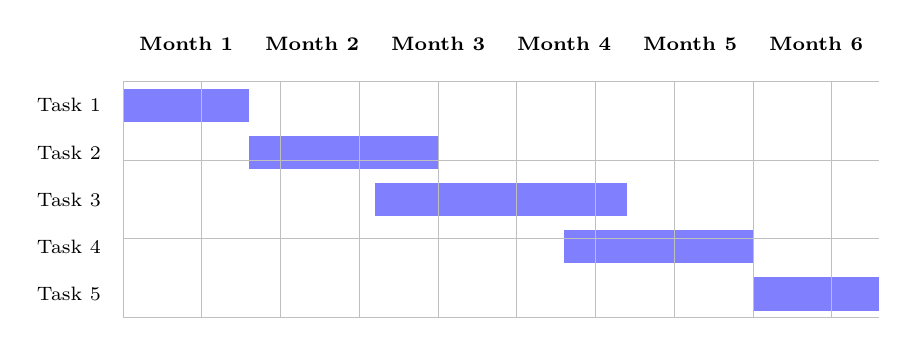
\begin{tikzpicture}[x=1.6cm,y=0.6cm]
    % Month headers (edit as needed)
    \foreach \m [count=\i from 0] in {Month 1,Month 2,Month 3,Month 4,Month 5,Month 6}
      \node[font=\scriptsize\bfseries] at (\i+0.5,0.8) {\m};
    % Tasks: {name/start/duration}
    \foreach \t/\s/\d [count=\j] in {Task 1/0/1, Task 2/1/1.5, Task 3/2/2, Task 4/3.5/1.5, Task 5/5/1}{
      \node[anchor=east,font=\scriptsize] at (-0.1,-\j+0.5) {\t};
      \fill[blue!50] (\s,-\j+0.15) rectangle ++(\d,0.7);
    }
    \draw[gray!50] (0,0) grid (6,-5);
  \end{tikzpicture}
\end{frame}

% ============================================================
%  10. MAPPING WITH POs
% ============================================================
\begin{frame}{Mapping with Program Outcomes (POs)}
  \centering\small
  \begin{tabular}{@{}lcccccccccccc@{}}
    \toprule
    & PO1 & PO2 & PO3 & PO4 & PO5 & PO6 & PO7 & PO8 & PO9 & PO10 & PO11 & PO12 \\
    \midrule
    Project & & & & & & & & & & & & \\
    \bottomrule
  \end{tabular}

  \vspace{1em}
  \placeholder{Justification for mapping -- consult guide}
\end{frame}

% ============================================================
%  11. MAPPING WITH SDGs
% ============================================================
\begin{frame}{Mapping with Sustainable Development Goals (SDGs)}
  \begin{itemize}
    \item \textbf{SDG \placeholder{No.}:} \placeholder{Goal name -- justification}
    \item \textbf{SDG \placeholder{No.}:} \placeholder{Goal name -- justification}
  \end{itemize}
\end{frame}

% ============================================================
%  12. DESIGN DETAILS (5--7 slides)
% ============================================================
\section{Design Details}

\begin{frame}{Design Details: System Architecture}
  \centering
  \placeholder{Insert system architecture diagram}
\end{frame}

\begin{frame}{Design Details: Use Case Diagram}
  \centering
  \placeholder{Insert use case diagram}
\end{frame}

\begin{frame}{Design Details: Level 0 DFD}
  \centering
  \placeholder{Insert Level 0 DFD}
\end{frame}

\begin{frame}{Design Details: Level 1 DFD}
  \centering
  \placeholder{Insert Level 1 DFD}
\end{frame}

\begin{frame}{Design Details: Data Processing Flow}
  \centering
  \placeholder{Insert data processing flowchart}
\end{frame}

\begin{frame}{Design Details: Sequence Diagram}
  \centering
  \placeholder{Insert sequence diagram}
\end{frame}

\begin{frame}{Design Details: Circuit / Hardware Design}
  \centering
  \placeholder{Insert circuit / hardware design}
\end{frame}

% ============================================================
%  13. BACK END DETAILS WITH DESIGN (4--5 slides)
% ============================================================
\section{Back End Details}

\begin{frame}{Back End: Overview}
  \begin{itemize}
    \item \placeholder{Back-end architecture overview}
  \end{itemize}
\end{frame}

\begin{frame}{Back End: Database Design}
  \centering
  \placeholder{Insert ER diagram / schema}
\end{frame}

\begin{frame}{Back End: Data Flow \& Communication}
  \centering
  \placeholder{Insert communication / API design}
\end{frame}

\begin{frame}{Back End: Processing Logic}
  \centering
  \placeholder{Insert algorithm / flowchart}
\end{frame}

\begin{frame}{Back End: Storage \& Security}
  \begin{itemize}
    \item \placeholder{Point 1}
    \item \placeholder{Point 2}
  \end{itemize}
\end{frame}

% ============================================================
%  14. REFERENCES (APA format)
% ============================================================
\begin{frame}[allowframebreaks]{References}
  \small
  \begin{enumerate}
    \item[] \placeholder{Author, A. A., \& Author, B. B. (Year). Title of article.
      \textit{Journal Name, Volume}(Issue), pages. https://doi.org/xxxx}
    \item[] \placeholder{Reference 2}
    \item[] \placeholder{Reference 3}
  \end{enumerate}
\end{frame}

% ============================================================
%  THANK YOU
% ============================================================
\begin{frame}[plain]
  \centering\vfill
  {\Huge Thank You}\\[1em]
  {\large Questions?}
  \vfill
\end{frame}

\end{document}
